\documentclass{article}

\usepackage[utf8]{inputenc}
\usepackage{blindtext}
\usepackage{graphicx}
\usepackage{float} % Elimina la condicion de flotante de las imagenes
\usepackage[english, activeacute]{babel}
\usepackage{amsmath}
\usepackage{etoolbox,fancyhdr,xcolor} % Colores
\usepackage[hidelinks]{hyperref} % Indice dinámico
\usepackage[a4paper]{geometry}
\usepackage{listings} % Para mostrar fragmentos de código.
\usepackage{multicol}
\usepackage[lighttt]{lmodern}

\title{Assignment 2.}
\author{José Manuel Izquierdo Ramírez}

\newcommand{\headrulecolor}[1]{\patchcmd{\headrule}{\hrule}{\color{#1}\hrule}{}{}}
\newcommand{\footrulecolor}[1]{\patchcmd{\footrule}{\hrule}{\color{#1}\hrule}{}{}}
\pagestyle{fancy}
\fancyhf{}% Clear header/footer
\fancyhead[L]{\textsl{\leftmark}}
\fancyfoot[C]{\thepage}% \fancyfoot[R]{\thepage}
\renewcommand{\headrulewidth}{0.4pt}% Default \headrulewidth is 0.4pt
\renewcommand{\footrulewidth}{0.4pt}% Default \footrulewidth is 0pt
\headrulecolor{cyan!70}% Set header rule colour to 70% red.
\footrulecolor{cyan!70}
\renewcommand{\sectionmark}[1]{\markboth{#1}{}}
\renewcommand{\subsectionmark}[1]{\markright{#1}}

% Multicol
\setlength{\columnseprule}{0.4pt}
\def\columnseprulecolor{\color{cyan!70}}

% Anular el sangrado
%\setlength{\parindent}{0cm}


\lstset{basicstyle=\ttfamily, keywordstyle=\bfseries}


\begin{document}

    \begin{titlepage}
        
        \centering
        {\LARGE\bfseries Assignment 2. \par}
        \vspace{0,5cm}
        {\itshape\Large Metaheuristics \par}
        \vspace{0,5cm}        
        \vspace{1cm}
        
\includegraphics[width=0.6\textwidth]{../media/Logo_UCO.png}\par
        \vspace{3cm}
        {\LARGE\bfseries José Manuel Izquierdo Ramírez \par}

        %{\large \today\par}

    \end{titlepage}
    
    \begin{index}
        \tableofcontents
        \newpage
        \listoffigures
    \end{index}

    \newpage
    
    \section{Exercise 1.}
    \subsection*{How does the algorithm behave as we modify the number of solutions, generations, tournament size, crossover probability, and mutation probability? Add more objects to the problem to check the behavior of the algorithm.}
    \subsection{Choosing a complex problem.}

    To perform these measurements we will first start by evaluating the behaviour of the algorithm when we add more objects.
    We add more objects in order to evaluate the behaviour of the algorithm when solving a sufficiently complex problem.
        
    We will start by evaluating 100 times each entry of the dataset reflected in the input.txt file, which contains 5,6,7,8,10,15 and 24 items.

        \begin{figure}[H]

            \centering
            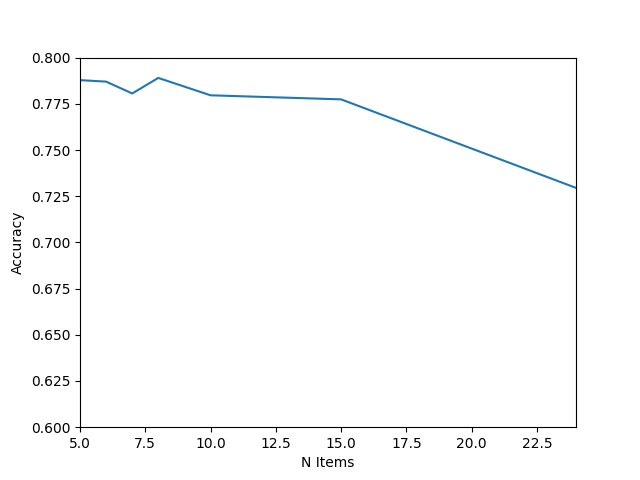
\includegraphics[width=0.75\textwidth]{../media/ej1/00.accuracy_items_change.png}
            \caption{Accuracy when the number of items increase}
            \label{Accuracy when the number of items increase}

        \end{figure}

        A visual analysis shows that the accuracy decreases as the number of items increases,
        Pearson's correlation coefficient corroborates this, as the relationship between both variables 
        is -0.93 with a certainty of 99.7\%.

        Next we will evaluate the behaviour of the metaheuristic when we modify each of the hyperparameters, 
        these will be evaluated for the following problem:

        \begin{itemize}
            \item Max Weight = 6404180
            \item Weights = [382745,799601,909247,729069,467902, 44328, 34610,698150,823460,\\
            903959,853665,551830,610856,670702,488960,951111,323046,446298,931161,31385,496951,\\
            264724,224916,169684]
            \item Prices = [825594,1677009,1676628,1523970,943972,97426,69666,1296457,1679693,1902996,\\
            1844992,1049289,1252836,1319836, 953277,2067538, 675367, 853655,1826027,  65731, 901489,\\
             577243, 466257, 369261]
        \end{itemize}

    \subsection{Analyzing the behavior when we modify the hyperparameters.}

    To analyse the behaviour we will carry out 100 iterations for each of the values of each hyperparameter.
    We will analyse the accuracy, mean, variance and standard deviation of the knapsack value and the Pearson's correlation coefficient between accuracy
    and the hyperparameter in particular.

    \subsection*{Modifying the number of solutions}

    \begin{figure}[H]

        \centering
        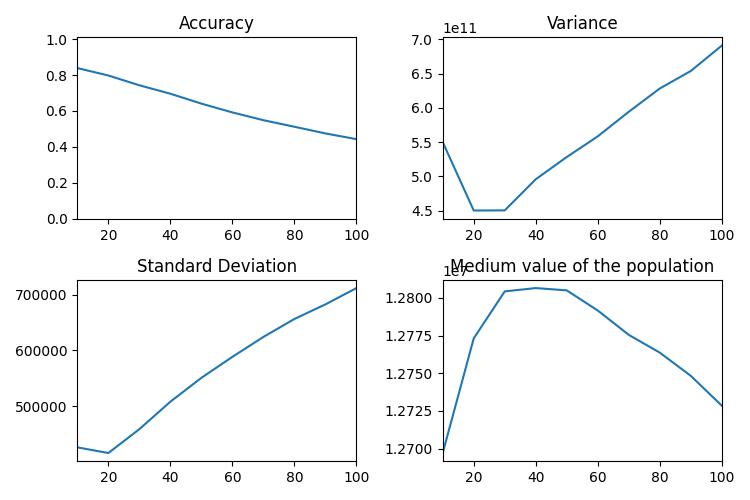
\includegraphics[width=1\textwidth]{../media/ej1/01.NSolutions_behaviour.png}
        \caption{Statistics when we change the number of solutions}
        \label{Statistics when we change the number of solutions}

    \end{figure}

    Pearson's correlation coefficient indicates that the correlation is not statistically significant, 
    since the p-value result ($\simeq 1$) is well above the significance level. 

    From the graphs we can deduce that by increasing the number of solutions, the population, 
    we introduce more variance to the population, which causes the accuracy to drop as well as the mean of the population value.

    \subsection*{Modifying the maximum number of generations}

    \begin{figure}[H]

        \centering
        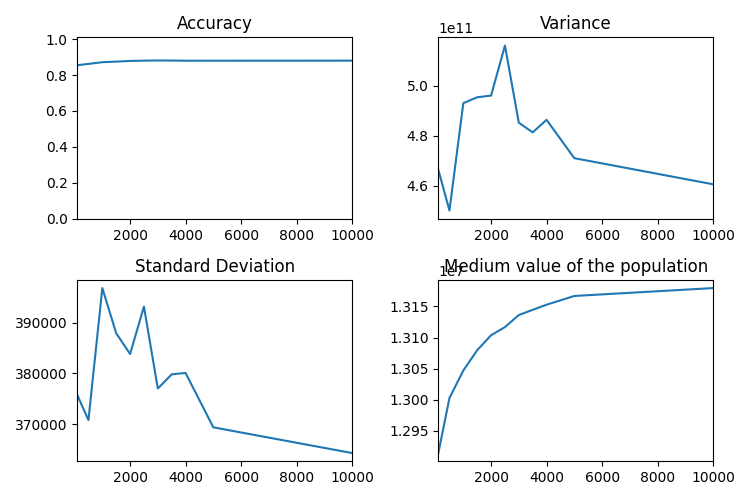
\includegraphics[width=1\textwidth]{../media/ej1/02.MaxGenerations_behaviour.png}
        \caption{Statistics when we change the maximum number of generations}
        \label{Statistics when we change the maximum number of generations}

    \end{figure}

    Pearson's correlation coefficient indicates that there is a moderate correlation (0.59) with a certainty of 94.8\%,
    This indicates that both variables will have the same tendency, if the number of generations increases, the accuracy will increase.
    not hardly perceptible but it is undergoing slight increases in the graph.

    The variance and standard deviation graphs show how they decrease as the maximum number of generations increases.

    The population mean grows exponentially, this may be because the population is converging to the optimal solution.

    \subsection*{Modifying the tournament size}

    \begin{figure}[H]

        \centering
        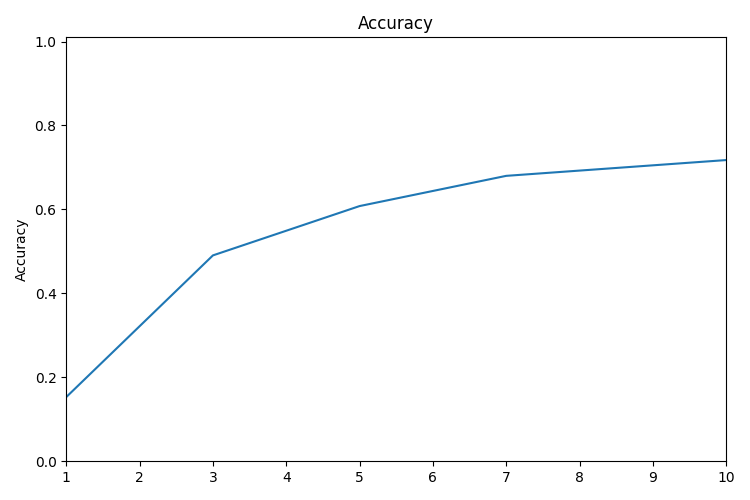
\includegraphics[width=0.75\textwidth]{../media/ej1/03.TournamentSize_behaviour.png}
        \caption{Statistics when we change the tournament size}
        \label{Statistics when we change the tournament size}

    \end{figure}

    For this section I have had some problems in representing the values of the mean, variance and standard deviation.

    \begin{lstlisting}[language=Python]
        
        import numpy as np
        
        ....

        mean = np.average(knapsack_values)
        var = np.var(knapsack_values)
        std = np.std(knapsack_values)    
        
    \end{lstlisting}

    This code for this case provides a Runtime Warning and the results it gives are nan.

    Pearson's correlation coefficient tells us that there is a strong correlation (0.88) with a certainty of 95.5\%.

    \subsection*{Modifying the crossover probability}

    \begin{figure}[H]

        \centering
        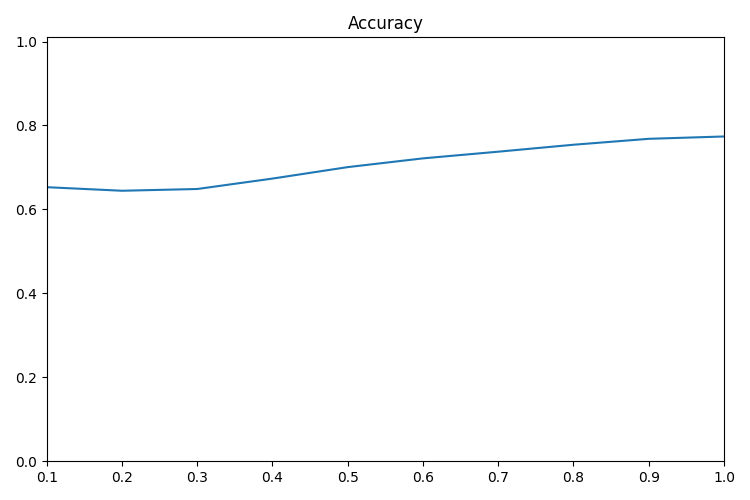
\includegraphics[width=0.75\textwidth]{../media/ej1/04.CrossoverProb_behaviour.png}
        \caption{Statistics when we change the probability of crossover}
        \label{Statistics when we change the probability of crossover}

    \end{figure}

    In this section I have had the same problem as in the previous one when obtaining the graphs of the variance, standard deviation and mean of the population.

    The Pearson correlation coefficient indicates that there is a strong correlation (0.97) with a certainty of 99.9\%.

    \subsection*{Modifying the mutation probability}

    \begin{figure}[H]

        \centering
        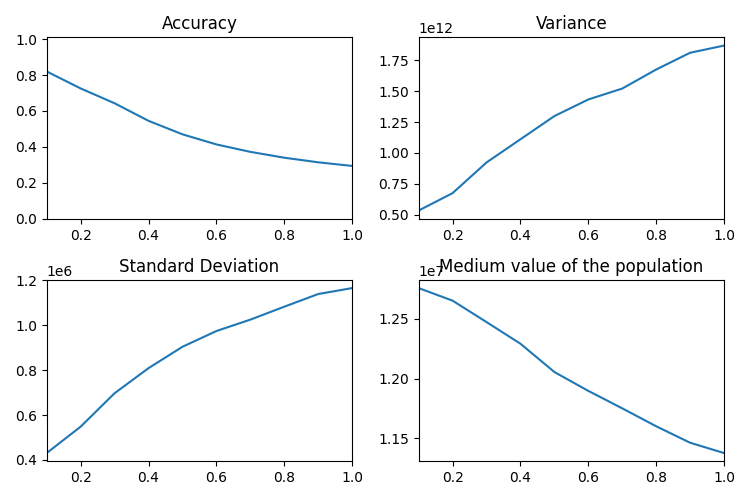
\includegraphics[width=1\textwidth]{../media/ej1/05.MutationProb_behaviour.png}
        \caption{Statistics when we change the probability of mutation}
        \label{Statistics when we change the probability of mutation}

    \end{figure}

    As the probability of mutation increases, areas further away from the most optimal area will be explored with a higher probability,
    This causes the accuracy to decrease, as well as the mean value of the population.
    The opposite happens, the variance and standard deviation increase because we are including individuals that are very different from the population.

    Pearson's correlation coefficient indicates that there is a strong correlation (-0.97) with a certainty of 99.9\%.
    indicates that as one of the variables increases, the other decreases.
        
    \subsection{Conclusions of the behavior of the algorithm}

    Taking into account the analysis carried out we can conclude what would be the ideal combination of hyperparemeters for our problem.

    For the number of solutions we can say that the ideal value is 20, where the accuracy is around 80\%, the variance and standard deviation reaches its minimum, and the population mean does not reach its maximum, but is very close.
    and the population mean does not reach its maximum, but it is very close.

    For the maximum number of generations we can say that the higher the value the better, as this will minimise the variance and standard deviation functions and maximise the mean value of the population. 
    Although the higher the value the better, we should be aware that these operations will require a lot of computational time, so we should establish a stopping criterion
    that takes into account, for instance, how much the algorithm has improved over the last few iterations and if this improvement is insignificant, stop.

    For the tournament size we would use a value of 10, as this gives us a higher accuracy.
    
    For the croosover probability we will use 1 or a value close to one, as these have the highest accuracy.

    For the mutation probability we would use a value the smaller the better, as this gives us a value of 80\% accuracy, a high population mean value and a small value for variance and standard deviation.


    \subsection{Do you always get the best solution? Why? What does it depend on?}

    No, the algorithm may converge prematurely to an area with good results, but not the best, to avoid this we can either
    increase the mutation probability, as this ensures that we will explore other areas of the search space, or we can apply elitism.
    
    It depends on the value assigned to the hyperparameters.

    \subsection{Modify the code to incorporate elitism. The best solution is kept in the elite and it
    is never lost until a new better one is obtained. This solution is the one that is
    returned at the end. Have you managed to improve? Why?}


    \subsection*{Modifying the number of solutions}

    \begin{figure}[H]

        \centering
        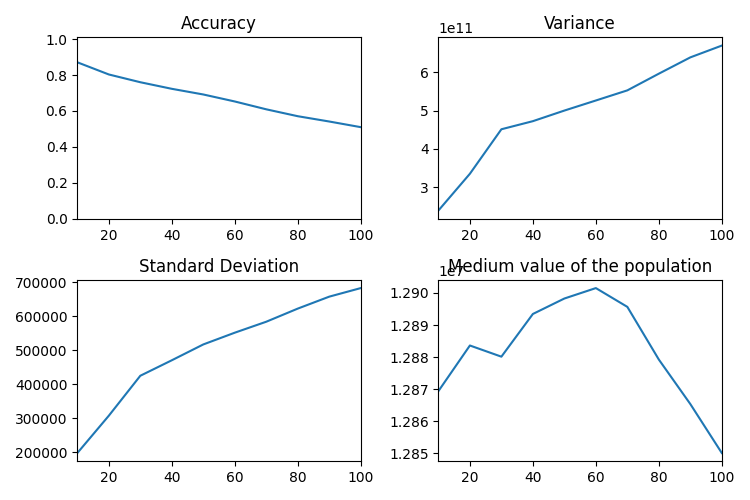
\includegraphics[width=1\textwidth]{../media/ej1/01.NSolutions_withElitism_behaviour.png}
        \caption{Statistics when we change the number of solutions and use elitism}
        \label{Statistics when we change the number of solutions and use elitism}

    \end{figure}

   
    \subsection*{Modifying the maximum number of generations}

    \begin{figure}[H]

        \centering
        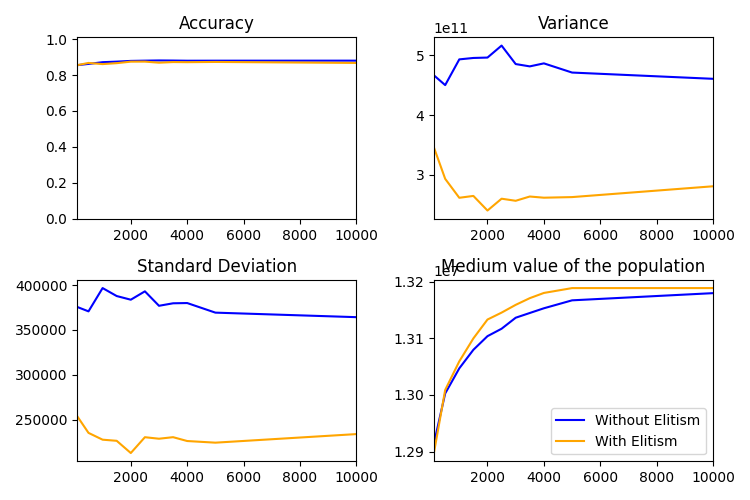
\includegraphics[width=1\textwidth]{../media/ej1/02.MaxGenerations_withElitism_behaviour.png}
        \caption{Statistics when we change the maximum number of generations and use elitism}
        \label{Statistics when we change the maximum number of generations and use elitism}

    \end{figure}

    
    \subsection*{Modifying the tournament size}

    \begin{figure}[H]

        \centering
        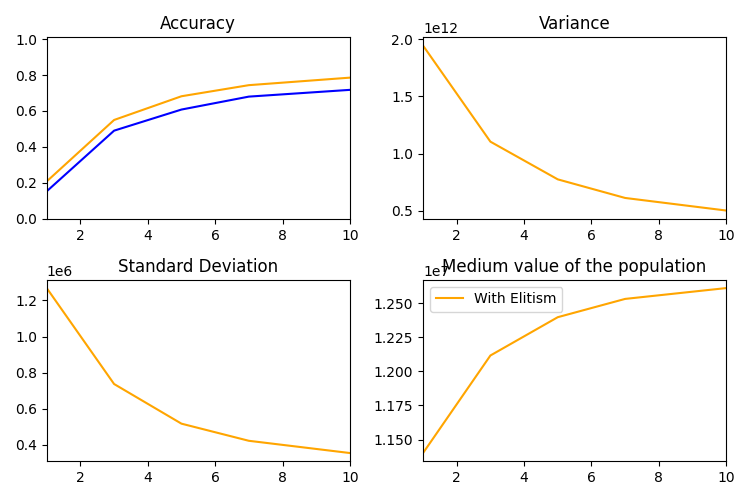
\includegraphics[width=1\textwidth]{../media/ej1/03.TournamentSize_withElitism_behaviour.png}
        \caption{Statistics when we change the tournament size and use elitism}
        \label{Statistics when we change the tournament size and use elitism}

    \end{figure}

    
    
    \subsection*{Modifying the crossover probability}

    \begin{figure}[H]

        \centering
        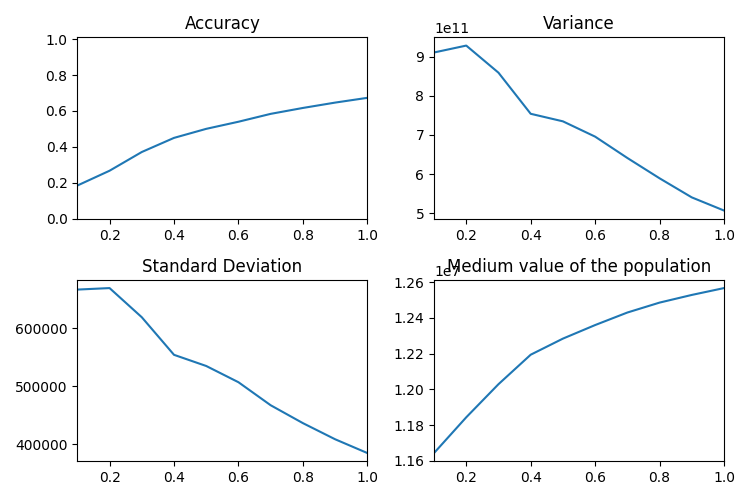
\includegraphics[width=1\textwidth]{../media/ej1/04.CrossoverProb_withElitism_behaviour.png}
        \caption{Statistics when we change the probability of crossover and use elitism}
        \label{Statistics when we change the probability of crossover and use elitism}

    \end{figure}

    
    \subsection*{Modifying the mutation probability}

    \begin{figure}[H]

        \centering
        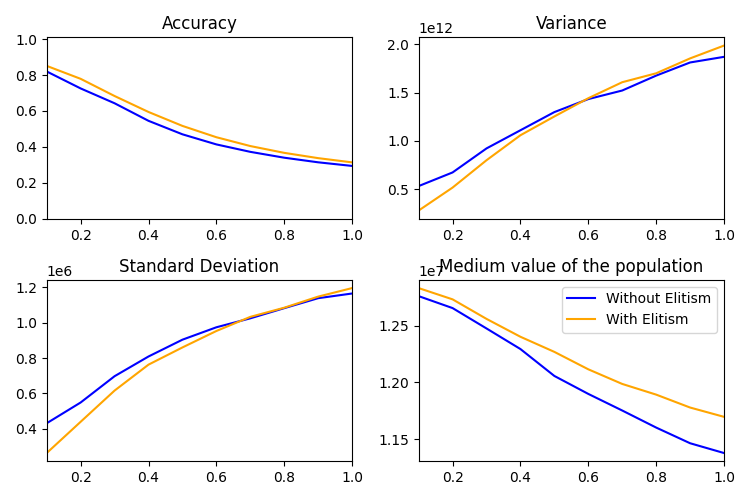
\includegraphics[width=1\textwidth]{../media/ej1/05.MutationProb_withElitism_behaviour.png}
        \caption{Statistics when we change the probability of mutation and use elitism}
        \label{Statistics when we change the probability of mutation and use elitism}

    \end{figure}

    \subsection{Conclusions of the behavior of the algorithm with elitism}

    In general, the accuracy value increases slightly, as does the mean value of the knapsack, and the variance and standard deviation curves smooth out.
    and the variance and standard deviation curves are smoothed.
    
    So, yes, the algorithm has been improved by applying elitism.

    \subsection{So far, we have started with valid solutions. Change it so that any solution can be
    generated. Does it affect the final performance? Analyze this issue.}


    \subsection*{Modifying the number of solutions}

    \begin{figure}[H]

        \centering
        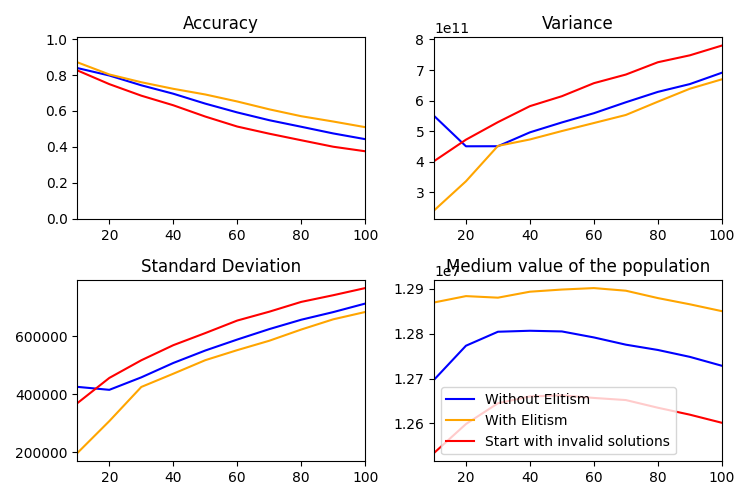
\includegraphics[width=1\textwidth]{../media/ej1/01.NSolutions_withInvSols_behaviour.png}
        \caption{Statistics when we change the number of solutions and start with invalid solutions}
        \label{Statistics when we change the number of solutions and start with invalid solutions}

    \end{figure}

   
    \subsection*{Modifying the maximum number of generations}

    \begin{figure}[H]

        \centering
        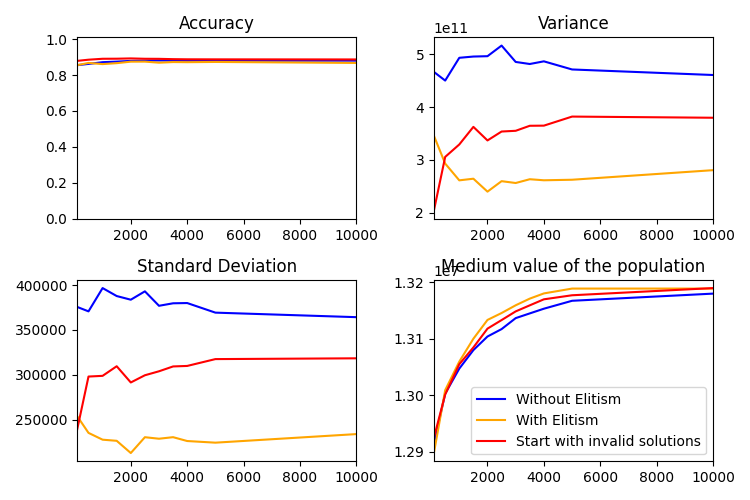
\includegraphics[width=1\textwidth]{../media/ej1/02.MaxGenerations_withInvSols_behaviour.png}
        \caption{Statistics when we change the maximum number of generations and start with invalid solutions}
        \label{Statistics when we change the maximum number of generations and start with invalid solutions}

    \end{figure}

    
    \subsection*{Modifying the tournament size}

    \begin{figure}[H]

        \centering
        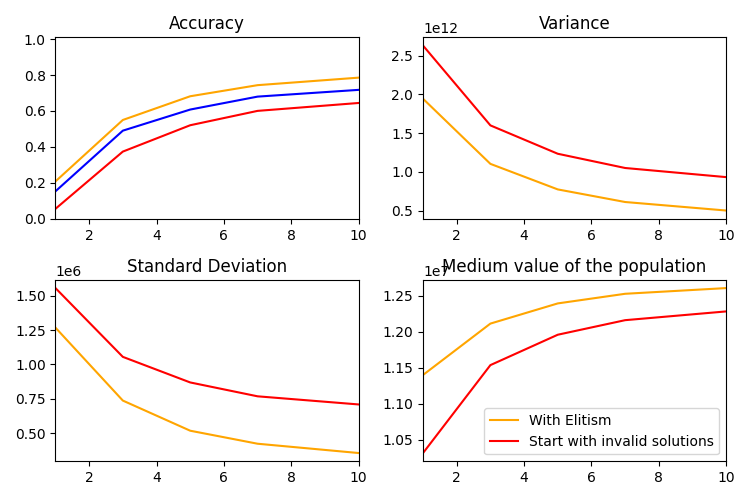
\includegraphics[width=1\textwidth]{../media/ej1/03.TournamentSize_withInvSols_behaviour.png}
        \caption{Statistics when we change the tournament size and start with invalid solutions}
        \label{Statistics when we change the tournament size and start with invalid solutions}

    \end{figure}

    
    
    \subsection*{Modifying the crossover probability}

    \begin{figure}[H]

        \centering
        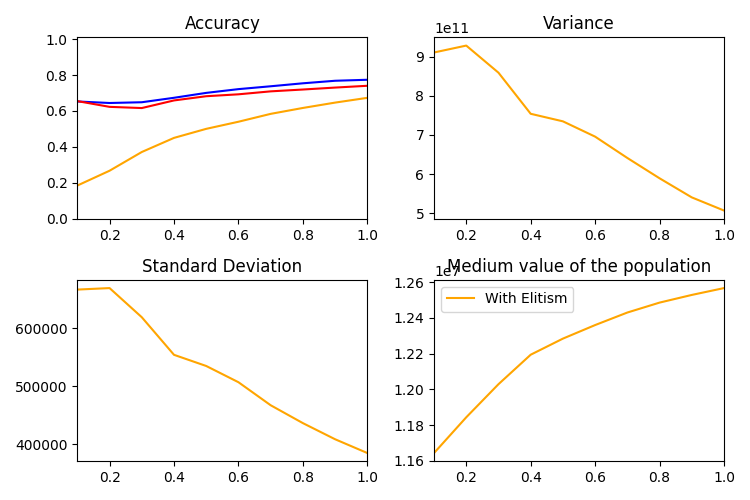
\includegraphics[width=1\textwidth]{../media/ej1/04.CrossoverProb_withInvSols_behaviour.png}
        \caption{Statistics when we change the probability and start with invalid solutions}
        \label{Statistics when we change the probability of crossover and start with invalid solutions}

    \end{figure}

    
    \subsection*{Modifying the mutation probability}

    \begin{figure}[H]

        \centering
        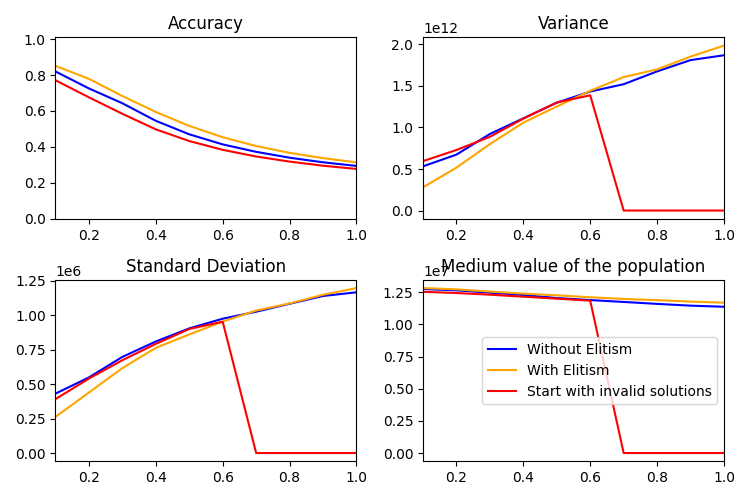
\includegraphics[width=1\textwidth]{../media/ej1/05.MutationProb_withInvSols_behaviour.png}
        \caption{Statistics when we change the probability of mutation and start with invalid solutions}
        \label{Statistics when we change the probability of mutation and start with invalid solutions}

    \end{figure}

    The graph falls down to 0 because the results for that probabilities are NaN.

    \subsection{Conclusions of the behavior of the algorithm with elitism}

    In general, the accuracy is smaller than the accuracy starting with valid solutions or using elitism, as same as the average value of
    the knapsack. On the other hand using invalid solutions increase the variance and the standard deviation.

\end{document}